\chapter{Project - Wavy Wall Analysis}\glsresetall
\section{Power Saved by the Wavy Wall (WW)}
With our definition of $P_\text{sav,\gls*{wv}}$ staying the same, we no longer believe it is equal to $P_\text{sav,\gls*{sl}}$. However, since we matched the periodic spanwise shear, we still maintain that the reduction in stochastic turbulent dissipation is the same between the \gls{ww} and \gls{ssl} flow, i.e. $\frac{\Delta \Phi _{\mathbf{u} ',\gls*{sl}}\pz}{\Phi _{0}\pz}=\frac{\Delta \Phi _{\mathbf{u} ',\gls*{wv}}\pz}{\Phi _{0}\pz}$. Therefore,
\begin{align}
	P_\text{sav,\gls*{wv}}	-P_\text{sav,\gls*{sl}} &= 100\%\frac{\Delta \Phi _{\overline{U },\gls*{wv}}\pz+\Delta \Phi _{\mathbf{u} ',\gls*{wv}}\pz}{\Phi \zz\pz}-100\% \frac{\Delta \Phi _{\overline{U },\gls*{sl}}\pz+\Delta \Phi _{\mathbf{u} ',\gls*{sl}}\pz}{\Phi \zz\pz}\\
	P_\text{sav,\gls*{wv}}	-P_\text{sav,\gls*{sl}}  &= 100\% \frac{\Delta \Phi _{\overline{U },\gls*{wv}}\pz-\Delta \Phi _{\overline{U },\gls*{sl}}\pz}{\Phi \zz\pz}\\
	P_\text{sav,\gls*{wv}} &= 100\% \frac{ \Phi _{\overline{U },\gls*{wv}}\pz-\Phi _{\overline{U },\gls*{sl}}\pz}{\Phi \zz\pz}+P_\text{sav,\gls*{sl}}
.\end{align}


\section{The Spatial Stokes Layer (SSL) Mean Velocity Profile}\label{sec:sslmean}
Since we do not know the shape of the \gls{ww} mean streamwise velocity profile to figure out dissipation due to the mean profile, we must start elsewhere. The \gls{ssl} mean streamwise velocity profile $\overline{U}\ssl\ps$ was given by \vqt, along with that of \gls{tsl}, the reference channel flow, and $\overline{U}^{+}=y^{+}$ for comparison (Figure~\ref{fig:sslmeanprofile}). We can see that at $y^{+}<10$, they all coincide to the linear profile $\overline{U}^{+}=y^{+}$, and at some point between $10<y^{+}<40$, they stop being curved on the logarithmic plot and become straight with similar slopes, indicating a logarithmic profile at higher $y^{+}$. In fact, like other \gls{dr} techniques (e.g. riblets), the \gls{dr} is noticeable as a thickening of the viscous sublayer causing an upward shift in this logarithmic portion of the mean velocity profile \cite{viotti2009,choi1989,luchini1996}. 

\begin{figure}[htbp]
	\centering
	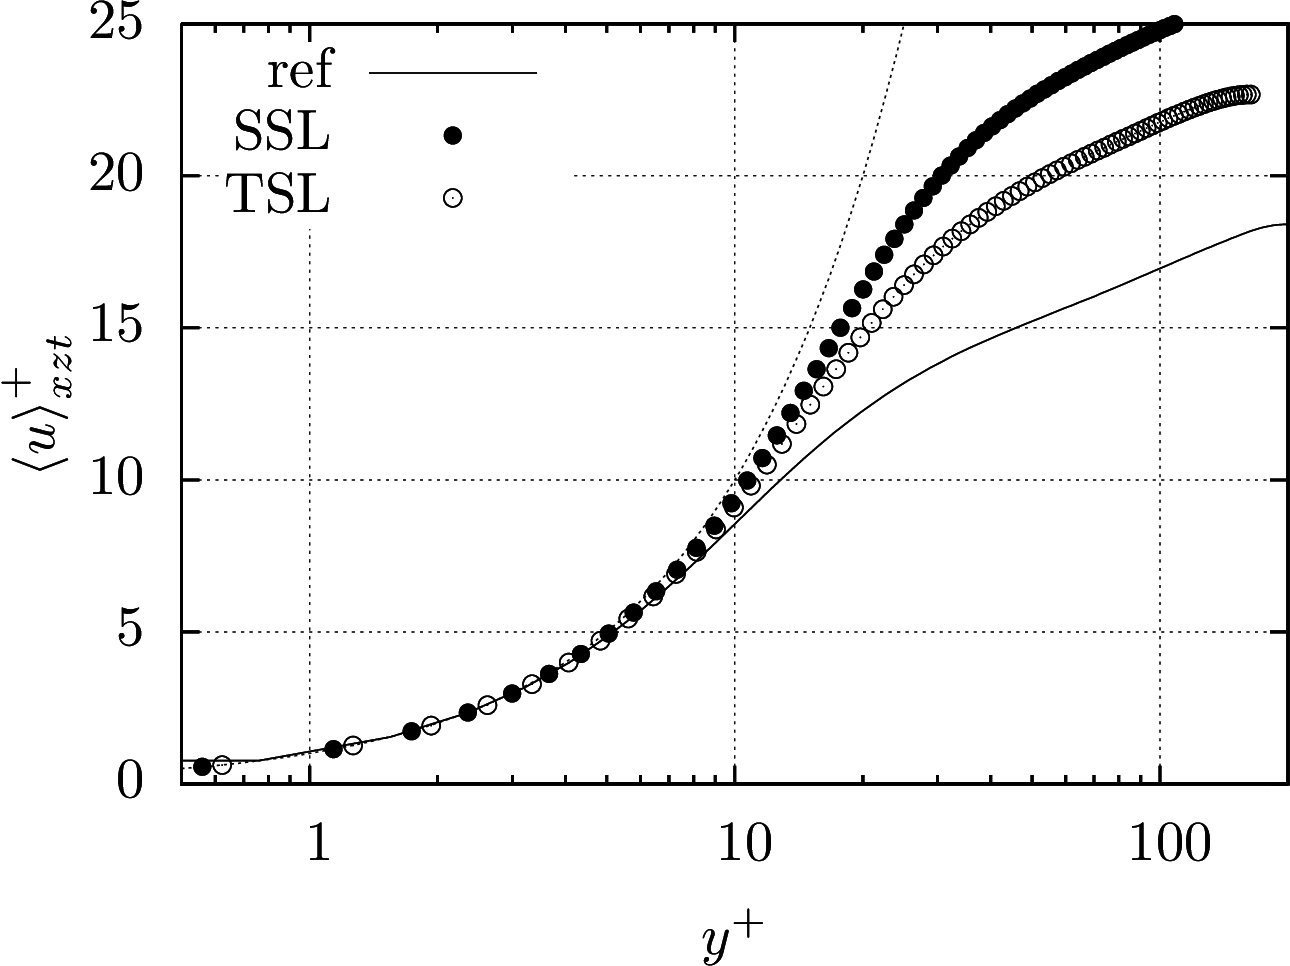
\includegraphics[width=0.7\linewidth]{project/fig/sslmeanprofile.png}
	\caption[Streamwise mean velocity profiles of SSL and reference flow]{Streamwise mean velocity profiles in wall units averaged in $x$-$z$ space, time, and phase ($\overline{U}^{+}\equiv \left<u \right>^{+}_{xzt}$) for \gls{ssl}, \gls{tsl}, the reference flow, and $\overline{U}^{+}=y^{+}$ (dotted line) for comparison \cite{viotti2009}.}
	\label{fig:sslmeanprofile}
\end{figure}

In order to see the differences more clearly, the  \gls{ssl} and refence flow data from Figure~\ref{fig:sslmeanprofile} were digitised using the web app webplotdigitiser. Then a curve fit was implemented and plotted in Figure~\ref{fig:sslmpcf} using an analytical fit for a turbulent plane channel flows given in an unpublished supplement to \cite{chernyshenko2021}. Abnormally, though, when the curve fit given for the mean streamwise velocity was used, the derivative thereof fluctuated much more than expected. Therefore, the curve fit for the second moments of velocity near the wall (root mean square velocity) was trialled instead, which produced much more reasonable derivative whilst also maintaining a good curve fit in and of itself. This latter curve fit is given as
\begin{equation}
	y^{+}  \frac{a\left(y^{+}\right)^2 + by^{+} + c}{q\left(y^{+}\right)^2 + ry^{+} + 1} + p \left( \ln(y^{+}+15)-\ln(15)\right)\label{eq:curvefit}
,\end{equation}
where $a,b,c,p,q,r$ are some coefficients. This function, however, does not guarantee that $\dv{U^{+}}{y^{+}} =1$ at the wall, which would be most accurate. We can see again that at $y^{+}<10$, the curves both fit on the $\overline{U}^{+}=y^{+}$ line. Then there is an area where the two curves diverge, but then, at around $y^{+}>60$, the gradients $\dv{\overline{U}^{+}}{y^{+}} $ seem to look fairly similar and in fact become negligible. This, as \textcite{viotti2009} had done, lead us to conjecture that the logarithmic portion of the \gls{ssl} mean velocity profile was the same as that of the reference flow but with an extra vertical shift.

Therefore, we take the well known logarithmic portion of the law of the wall, which applies to the reference flow,
\begin{equation} 
	\overline{U}\pz\zz=\frac{1}{\kappa}\ln y\pz+B\label{eq:cfref}
,\end{equation}
where $\kappa=0.41$, and  $B=5.0$ \cite{schlichting2016}, and add a vertical shift  $\Delta h$ to get
 \begin{equation}
	 \overline{U}\ps\ssl=\frac{1}{\kappa}\ln y\ps +B+\Delta h\ssl\label{eq:cfww}
.\end{equation}
$\Delta h$ can easily be estimated by drawing a straight line that follows the logarithmic portion of the \gls{ssl} mean profile (where $y^{+}>60$ ) on the logarithmic scale (in Figure~\ref{fig:sslmeanprofile}), reading the intercept of said straight line, and subtracting by $B$. By this method it was found that  $\Delta h\approx8$. Curve fits using Equations~\eqref{eq:cfref} and \eqref{eq:cfww} are plotted in Figure~\ref{fig:sslmpest}.

\begin{figure}[htbp]
	\centering
	\subfigure[Curve fits.]{
		\label{fig:sslmpcf}
        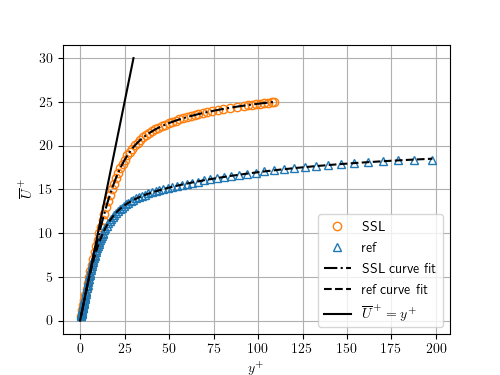
\includegraphics[width=0.485\linewidth]{project/fig/sslmeanprofilelin.png}}
	\subfigure[Estimated logarithmic profiles.]{
		\label{fig:sslmpest}
		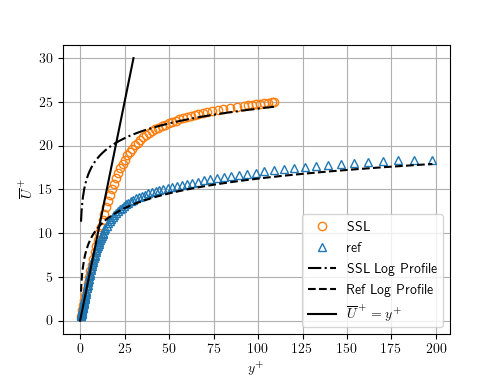
\includegraphics[width=0.485\linewidth]{project/fig/sslmeanprofileest.png}}
		\caption[Mean streamwise velocity profiles of SSL and reference flows, and analytical approximations thereof]{Both plots show data on the mean streamwise velocity profiles of \gls{ssl} (orange-circle) and the reference flow (blue-triangles) which were digitised from \textcite{viotti2009} (shown in Figure~\ref{fig:sslmeanprofile} and plotted on a linear scale, as well as $\overline{U}^+=y^+$ (solid-line). }
	\label{fig:sslmplin}
\end{figure}
The validity of using the same logarithmic profile with vertical shift as an estimate can be further seen in Figure~\ref{fig:sslmpdiff}, where the squares of the derivatives of the curvefits found using Equation~\eqref{eq:curvefit} were plotted for the \gls{ssl} and reference flows. We can see that the differences in the derivatives are negligibly small. Moreover, since dissipation is equal to the integral of this derivative from 0 to infinity, we can see that contributions at $y^{+}>60$ are negligible. Whilst we can only numerically integrate the curve fitted solution, we can actually analytically integrate the estimated solution as
\begin{align}
	\Phi _{\overline{U}}^{+} &= \int_{0}^{y_{\times}^{+}} \left| \frac{dy^{+}}{dy^{+}} \right|^2dy^{+} + \int_{y_{\times}^{+}}^{\infty} \left| \frac{d\left( \frac{1}{\kappa}\ln y^{+} +B+\Delta h\right) }{dy^{+}} \right|^2dy^{+}  \\
	&= \int_{0}^{y_{\times}^{+}} 1dy^{+} + \frac{1}{\kappa^2}\int_{y_{\times}^{+}}^{\infty} \left| \frac{1}{y^{+}} \right|^2dy^{+}  \\
	&= y_{\times}^{+} + \frac{1}{\kappa^2}\frac{1}{y_{\times}^{+}}\\
	&=\frac{\left(  \kappa y_{\times}^{+}  \right) ^2+ 1}{\kappa^2 y_{\times}^{+}}\label{eq:fiycross}
,\end{align}
where \gls*{ycrs} is the single point at which the linear profile crosses the logarithmic profile. For \gls{ssl}, we have We find that for this estimated profile, the ratio $\frac{\Phi _{\overline{U},\gls*{sl}}\ps}{\Phi _{\overline{U},\gls*{zer}}\pz}\rvert_\text{est}=1.818$, whereas the same ratio for the curve fitted profile $\frac{\Phi _{\overline{U},\gls*{sl}}\ps}{\Phi _{\overline{U},\gls*{zer}}\pz}\rvert_\text{cfit}=1.650$. The estimated ratio is only 10.1\% higher than that of the curve fitted solution. Therefore, the idea is that perhaps if we could model the mean profile of the \gls{ww} using the linear plus logarithmic profile approach, perhaps it would be good enough to measure the net power reduction of the \gls{ww} flow.
\begin{figure}[htbp]
	\centering
	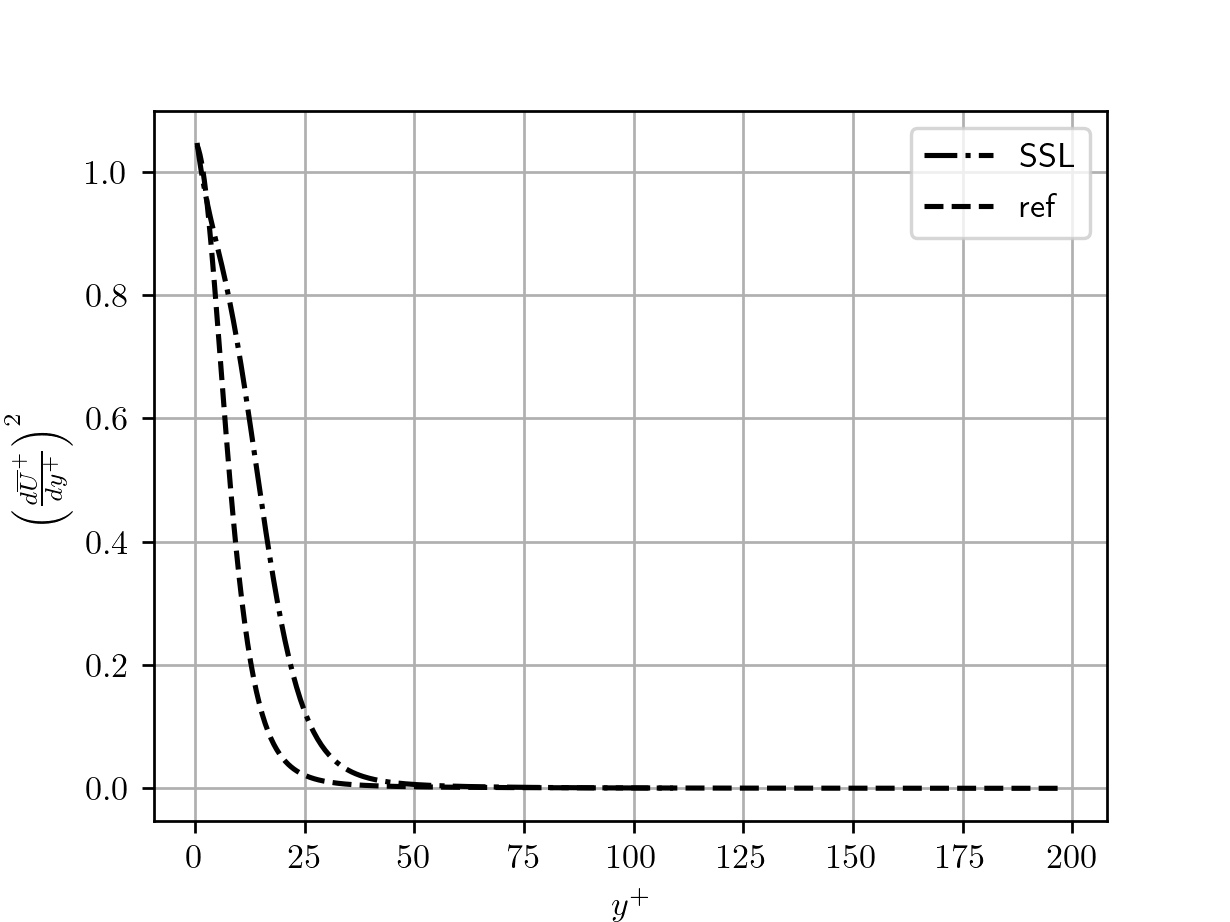
\includegraphics[width=0.7\linewidth]{project/fig/sslmeandiff.png}
	\caption[Mean streamwise shear profile squared of SSL and reference flows]{The squared mean streamwise shear profiles of \gls{ssl} (dot-dash), and reference (dash) flows, i.e. the squared derivative of mean streamwise velocity profiles $\dv{\overline{U}^{+}}{y^{+}} $ obtained using Equation~\eqref{eq:curvefit} for $\overline{U}^{+}$, which is shown in Figure~\ref{fig:sslmpcf}.}
	\label{fig:sslmpdiff}
\end{figure}

\section{Modelling the Wavy Wall (WW) Mean Velocity Profile}
With Equation~\eqref{eq:cfww}, \textcite{luchini1996} wrote that ``an increment in [$B$ i.e.  $\Delta h$] can be quantitatively translated into drag reduction because [$B$ ] appears explicitly in the drag formulae that'' since we can just integrate the mean velocity profile. For a turbulent boundary layer over a flat plate, the friction formula is given by
\begin{equation}
	\left( \frac{C_f}{2} \right) ^{-1 /2} = \frac{1}{\kappa}\ln \left[ \left( \frac{C_f}{2} \right) ^{1 /2 } \Rey_D \right] + 2.2 + B
,\end{equation}
where $\Rey_D $ is based on the velocity boundary-layer thickness \cite{white1991}. It turns out that for small increments in $B$,
 \begin{equation}
	 \frac{\Delta C_f}{C_{f,\gls*{zer}}}=-\frac{\Delta h}{\left(2C_{f,\gls*{zer}}\right)^{-1 /2} +\kappa /2}
,\end{equation}
where $\Delta C_f=C_f-C_{f,\gls*{zer}}$ \cite{luchini1996}. For \gls{ww}, $P_\text{net,\gls*{wv}} \equiv100\% \frac{C_{f,\gls*{zer}-C_{f,\gls*{wv}}}}{C_{f,\gls*{zer}}}$. Therefore,
\begin{align}
	-\frac{P_\text{net,\gls*{wv}}}{100\%} &=-\frac{\Delta h\ww}{(2C_{f,\gls*{zer}})^{-1 / 2}+\kappa / 2}\\
	\Delta h\ww &= \frac{P_\text{net,\gls*{wv}}}{100\%\left[(2C_{f,\gls*{zer}})^{-1 / 2}+\kappa / 2\right]}
.\end{align}
Thus, we believe the \gls{ww} mean velocity profile can be modelled by
\begin{equation}
	\overline{U}\ww\pw =
	\begin{cases}
		y\pw, & y\pw\leq y_{\times}\pw\\
		\frac{1}{\kappa}\ln y\pw +B +\frac{P_\text{net,\gls*{wv}}}{100\%\left[(2C_{f,\gls*{zer}})^{-1 / 2}+\kappa / 2\right]}, & y\pw>y_{\times}\pw
	\end{cases}
.\end{equation}

By modelling the \gls{ww} mean velocity profile like so, we can find $P_\text{net,\gls*{wv}} $ as only a function of $y_{\times}\pw$ by solving the two cases as a system of equations, i.e. we let $\overline{U}\ww\pw=y\pw$ in the logarithmic profile as follows
\begin{align}
	\overline{U}\pw\ww &=\frac{1}{\kappa}\ln y\pw +B +\frac{P_\text{net,\gls*{wv}}}{100\%\left[(2C_{f,\gls*{zer}})^{-1 / 2}+\kappa / 2\right]} \\
	y_\times\pw &=\frac{1}{\kappa}\ln y_\times\pw +B +\frac{P_\text{net,\gls*{wv}}}{100\%\left[(2C_{f,\gls*{zer}})^{-1 / 2}+\kappa / 2\right]} \\
	P_\text{net,\gls*{wv}} &=100\left(  y_{\times}\pw - \frac{1}{\kappa}\ln y_{\times}\pw - A \right) \left( (2C_{f,0})^{-\frac{1}{2}} +\frac{\kappa}{2} \right) 
.\end{align}

Moreover, we can also employ Equation~\eqref{eq:fiycross} combined with the wall unit conversions just as Equation~\eqref{eq:fislconv} to get
\begin{equation}
	\Phi _{\overline{U},\gls*{wv}}\pz = \Phi _{\overline{U},\gls*{wv}}\pw \left( \frac{\tau_{w,\gls*{wv}}}{\tau_{w,\gls*{zer}}} \right) ^{3 /2 }=\frac{\left(  \kappa y_{\times}^{+}  \right) ^2+ 1}{\kappa^2 y_{\times}^{+}} \left(  \frac{\tau_{w,\gls*{wv}}}{\tau_{w,\gls*{zer}}} \right) ^{3 /2 } \label{eq:fiwwpzycr}
.\end{equation}

But there is a slight problem here. Previously, for $\frac{\tau_{w,\gls*{sl}}}{\tau_{w,\gls*{zer}}}$, we have simply said this is equal to $1-\frac{P_\text{sav,\gls*{sl}}}{100\%} $ in an \gls{ssl} flow. However, in a \gls{ww} flow, this is not necessarily the case. $\tau_w$ only involves the frictional drag of the flow (the wall shear stress), but leaves out pressure drag which is present in the  \gls{ww} due to the undulations which create pressure gradients. As of writing, the author knows of no way to extract $\frac{\tau_{w,\gls*{wv}}}{\tau_{w,\gls*{zer}}}$. The only solution was to turn to \gls{dns} by \sgt. Through their results we were able to find that although the drag reduction and pressure drag reduction were of the same order, the pressure drag reduction was at least an order of magnitude smaller than the total drag, i.e. we conjecture that pressure drag on the \gls{ww} is $\ll \tau_{w,\gls*{wv}}$. Therefore, we let
\begin{equation}
	P_\text{net,\gls*{wv}}\approx 100\% \frac{\tau_{w,\gls*{zer}-\tau_{w,\gls*{wv}}}}{\tau_{w,\gls*{zer}}} \implies  \frac{\tau_{w,\gls*{wv}}}{\tau_{w,\gls*{zer}}}\approx1-\frac{P_\text{net,\gls*{wv}} }{100\%}\label{eq:tauassump}
,\end{equation}
even though it isn't necessarily true.

\section{Net Power Reduction by Wavy Wall (WW) - Results}
By accepting the assumption in Equation~\eqref{eq:tauassump}, quite accidentally, we have now stumbled upon a closed set of equations for which we can solve numerically for a given  $\lambda_x\pz$, $\lambda_z\pz$, and $\hat{W}\ssl\pz$. We start by recognising that nowhere in our analysis did we need to involve $P_\text{req,\gls*{wv}}=r_\text{min} P_\text{req,\gls*{sl}}  $. Therefore, $r_\text{min} $ stays the same, and $\frac{\lambda_x\pz}{\lambda_z\pz}\rvert_\text{opt} $ stays the same. Thus the closed set of equations is as follows
\begin{align}
	P_\text{net,\gls*{wv}} &= P_\text{sav,\gls*{wv}} + r_\text{min} P_\text{req,\gls*{sl}} \label{eq:Pnetww}\\  
	P_\text{sav,\gls*{wv}} &=  100\% \sqrt{\frac{C_{f,\gls*{zer}}}{2}}\left(  \frac{\left(  \kappa y_{\times,\gls*{wv}}\pw  \right) ^2+ 1}{\kappa^2 y_{\times,\gls*{wv}}\pw} \left( \frac{\tau_{w,\gls*{wv}}}{\tau_{w,\gls*{zer}}} \right) ^{\frac{3}{2}}-\Phi _{\overline{U},\gls*{sl}}\pz\right) +P_\text{sav,\gls*{sl}} \label{eq:Psavww}\\
	P_\text{net,\gls*{wv}} &=100\%\left(  y_{\times}\pw - \frac{1}{\kappa}\ln y_{\times}\pw- B \right) \left( (2C_{f,0})^{-\frac{1}{2}} +\frac{\kappa}{2} \right) \label{eq:ycross}\\
	P_\text{req,\gls*{sl}} &= -100\%\left( \hat{W}\pz  \right) ^2\sqrt{\frac{C_{f,\gls*{zer}}}{2}}   \left( \frac{2\pi (1-P_\text{sav,\gls*{sl}} / 100\%) }{\lambda_x\pz}\right) ^{\frac{1}{3}}\int_{0}^{\infty} \frac{1}{2} \left| \frac{d\check{w}\ps\ssl}{d\check{y}\ps} \right| ^2 d\check{y}\ps \\ 
		P_\text{sav,\gls*{sl}} &= f\left(\lambda_x\pz, \hat{W}\ssl\pz\right) \text{ (from Equation~\eqref{eq:psavsl})}\\
		\Phi _{\overline{U},\gls*{sl}}\pz &= \left( 1-\frac{P_\text{sav,\gls*{sl}} }{100\%} \right)  \left[\frac{\left(  \kappa y_{\times,\gls*{sl}}\ps  \right) ^2+ 1}{\kappa^2 y_{\times,\gls*{sl}}\ps}\right]\\
	y_{\times,\gls*{sl}}\ps&=\frac{1}{\kappa}\ln  y_{\times,\gls*{sl}}\ps +B+\Delta h\ssl \\
	C_{f,\gls*{zer}} &= 0.00336\Rey_{\tau}^{-0.273}
,\end{align}
where $\Delta h \ssl=8$, $\Rey_{\tau} = 200$,  $\kappa=0.41$,  $B=5.0$,  $r_\text{min} =5.846$, and $\int_{0}^{\infty} \frac{1}{2} \left| \frac{d\check{w}\ps\ssl}{d\check{y}\ps} \right| ^2 d\check{y}\ps = 0.3157$.

We solved this for $P_\text{net,\gls*{wv}} $ as a function of $\lambda_x\pz$ for $\hat{W}\ssl\pz=1,2,6,12$ and plotted them in Figure~\ref{fig:pnetww}. The code for solving these equations, as well as others in this report, along with many of the figures generated is in Appendix~\ref{app:code}.
\begin{figure}[htbp]
	\centering
	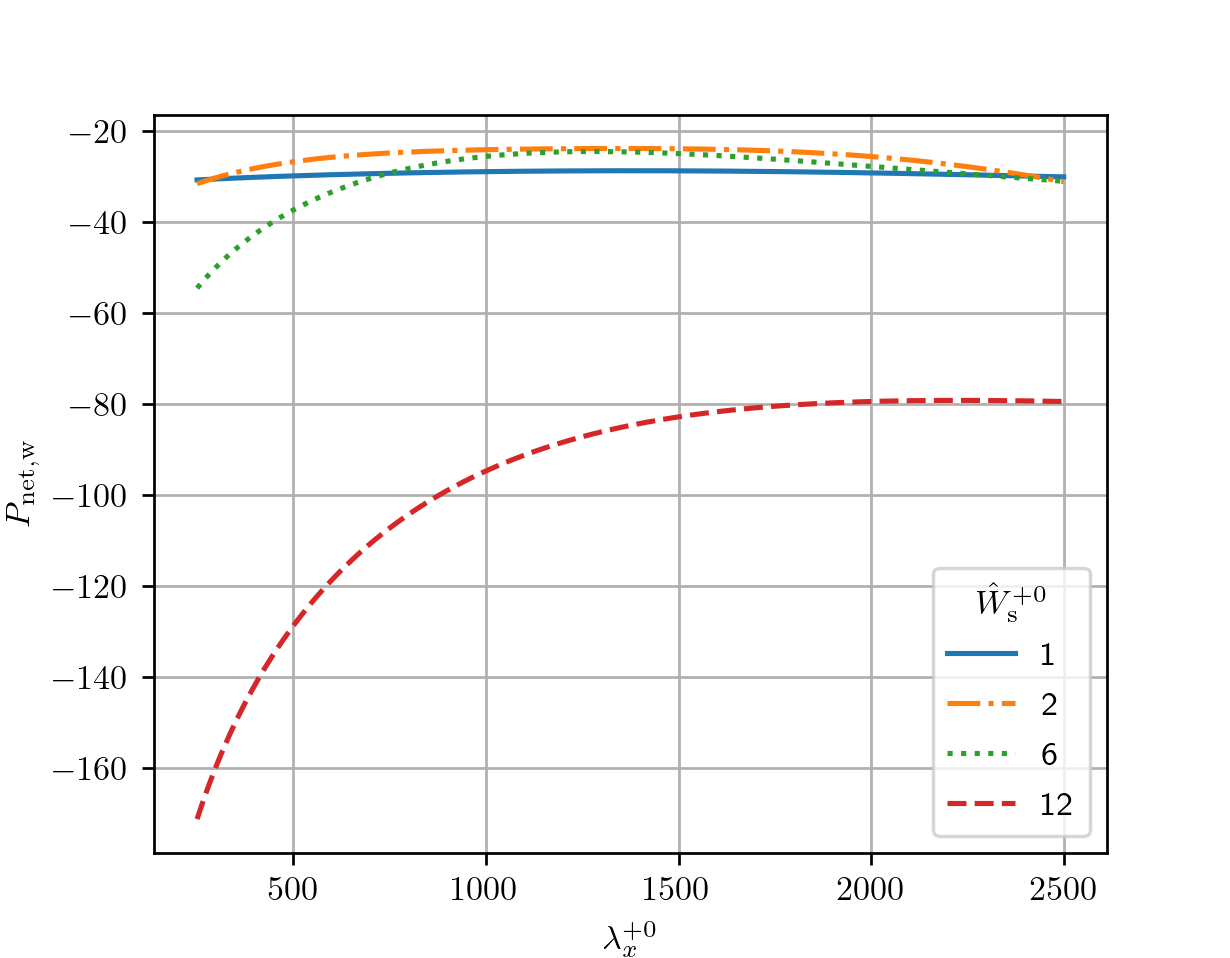
\includegraphics[width=0.7\linewidth]{project/fig/pnetww.png}
	\caption[Net power reduction for the wavy wall $P_\text{net,w}$]{Calculated net power reduction $P_\text{net,\gls*{wv}} $ for the wavy wall $P_\text{net,\gls*{wv}} $.}
	\label{fig:pnetww}
\end{figure}
